\documentclass[zavrsnirad]{fer}
\title{Object Localization in Images Using Deep Learning}
	\naslov{Lokalizacija objekata u slikama korištenjem dubokog učenja}
\brojrada{1606}
\author{Dominik Barukčić}
\date{June, 2021}
\datum{lipanj, 2021.}
\begin{document}
	\maketitle
	\zadatak{hr_0036538320_73.pdf}
	\begin{zahvale}
		zahvale
	\end{zahvale}
	\mainmatter
	\tableofcontents
	
	
	% TEKST RADA
	
	%--- UVOD / INTRODUCTION -------------------------------------------------------
	\chapter{Uvod}
	\label{pog:uvod}
	
	Neki od radova koje ćemo citirati su \cite{6248073,6247753,ghiglia_pritt_phase_unwrapping,hartley2003multiple,4250461,123DCatch}.
	Trebaju nam samo radi testiranja kako izgleda referenciranje rada s konferencije, rada iz časopisa, knjige i Internetske stranice.
	
	\begin{figure}[htb]
		\centering
		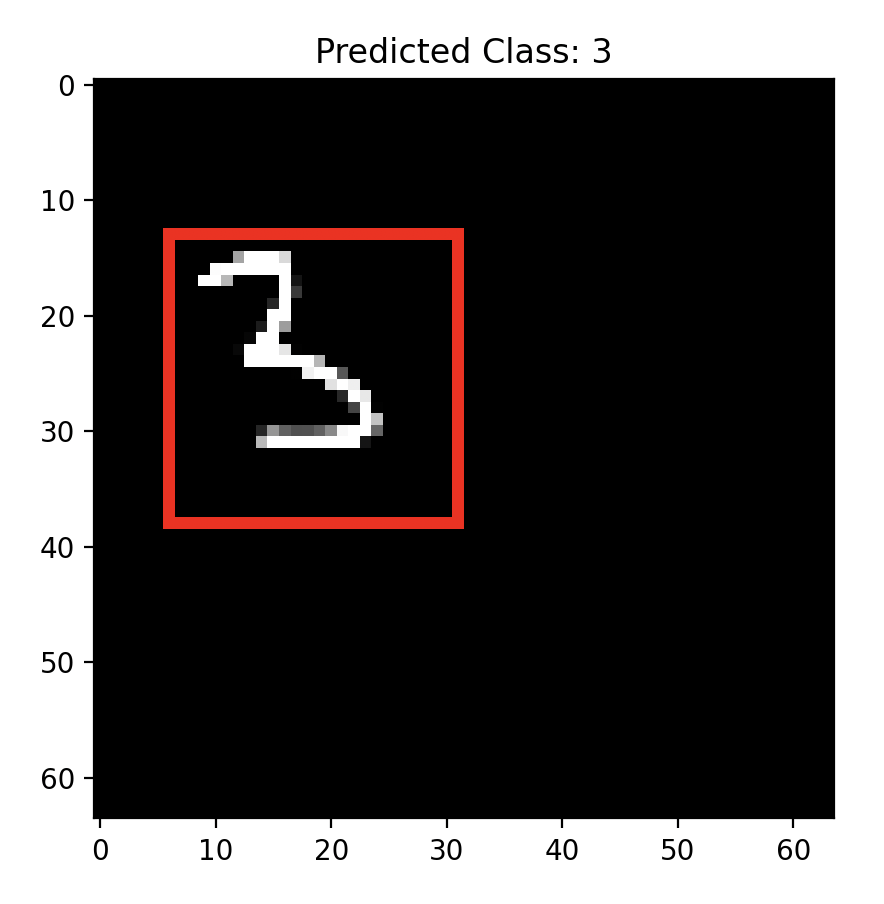
\includegraphics[width=0.38\linewidth]{Figures/primjer.png} 
		\caption{Moja prva slika}
		\label{slk:prvaslika}
	\end{figure}
	
	Referenciramo se na sliku \ref{slk:prvaslika} u sredini rečenice, zatim prije zareza \ref{slk:prvaslika}, te zatim na kraju rečenice \ref{slk:prvaslika}.
	Upravo smo testirali radi li naredba \verb|\ref| ispravno u slučaju kada nakon nje slijedi točka.
	
	Sada slijedi jedna jednadžba:
	\begin{equation}
		\label{jed:prvajednadzba}
		\int_{-\infty}^{+\infty}f(t)\,dt=F(\omega)
	\end{equation}
	Jednadžba \eqref{jed:prvajednadzba} je moja prva jednadžba koja defnira par $f(t)\ufrek F(\omega)$ ili $F(\omega)\uvrem f(t)$.
	
	
	%-------------------------------------------------------------------------------
	\chapter{Glavni dio}
	\label{pog:glavni_dio}
	
	Text
	
	
	%-------------------------------------------------------------------------------
	\chapter{Rezultati i rasprava}
	\label{pog:rezultati_i_rasprava}
	
	Text
	
	
	%--- ZAKLJUČAK / CONCLUSION ----------------------------------------------------
	\chapter{Zaključak}
	\label{pog:zakljucak}
	
	Text
	
	
	% literatura/references
	\bibliography{literatura}
	
	% sazetak/abstract
	\begin{sazetak}
		sažetak na hrvatskom
	\end{sazetak}
	\begin{kljucnerijeci}
		ključne riječi na hrvatskom
	\end{kljucnerijeci}
	\begin{abstract}
		abstract in English
	\end{abstract}
	\begin{keywords}
		keywords in English
	\end{keywords}
	
	% privitci/appendix
	\backmatter
	\chapter{The Code}

\end{document}